% Hasta acá tenemos definido como funciona el motor con una f
% Y como se transforma la posición en un input para la red

\section{\reflectbox{NNUE} (NNUE)}

\begin{frame}
\vfill
\centering
\begin{beamercolorbox}[sep=8pt,center,shadow=false,rounded=false]{title}
    \reflectbox{NNUE}: \textbf{E}fficiently \textbf{U}pdatable \textbf{N}eural \textbf{N}etworks
    \usebeamerfont{title}\par%
\end{beamercolorbox}
\vfill
\end{frame}

\begin{frame}
\frametitle{\reflectbox{NNUE}: \textbf{N}eural \textbf{N}etwork}
Ya tenemos definido el input* y el output: \pause
\begin{itemize}
\item El input es un vector one-hot generado por el \textit{feature set}. \pause
\item El output es un número real.
\end{itemize}
%\pause
%*: los feature sets dependen de la perspectiva!
\end{frame}


\begin{frame}
\frametitle{\reflectbox{NNUE}: \textbf{N}eural \textbf{N}etwork}
La red es una \textit{feedforward} clásica de 3 layers fully connected.
\begin{itemize}
    \item con activaciones ClippedReLU
    \item es siamés en la primera capa
\end{itemize}
\end{frame}

\begin{frame}
\frametitle{\reflectbox{NNUE}: \textbf{N}eural \textbf{N}etwork}
\begin{figure}[H]
\centering
\makebox[\textwidth]{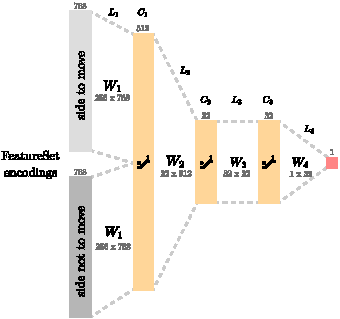
\includegraphics[width=6.5cm]{../assets/nnue/network.pdf}}
%\caption{Neural network architecture with $\bm{|S_P|}=768$, $\bm{L1}=256$, $\bm{L2}=32$. Not to scale.}
\end{figure}
\end{frame}

\begin{frame}
\frametitle{\reflectbox{NNUE}: \textbf{E}fficient \textbf{U}pdates (primera capa)}
\begin{figure}[H]
\centering
\subfloat[\centering Linear layer]{{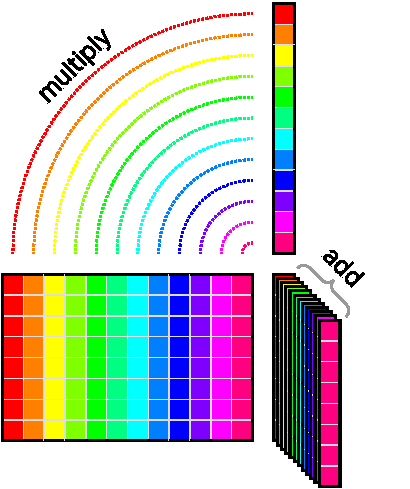
\includegraphics[width=4cm]{../assets/nnue/mv.pdf} }}%
\qquad
\subfloat[\centering Linear layer with sparse inputs]{{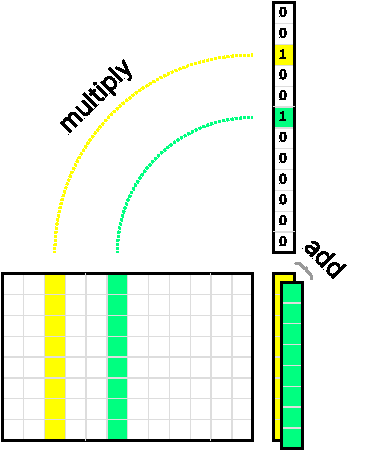
\includegraphics[width=4cm]{../assets/nnue/mvs.pdf} }}%
\caption{Linear layer operation comparison. Figures from [18].}
\end{figure}
\end{frame}

\begin{frame}
\frametitle{\reflectbox{NNUE}: Concatenación de la primera capa}
\begin{figure}[H]
\centering
\makebox[1.05\textwidth]{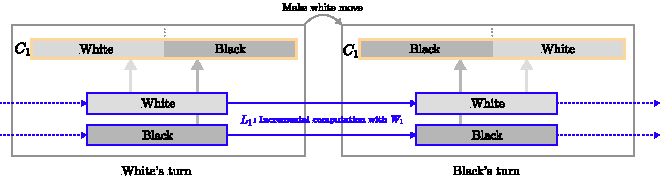
\includegraphics[width=1.05\textwidth]{../assets/nnue/incremental_update.pdf}}
\caption{Concatenation of the first layer's output after a move is made. Inspired by a CPW figure.}
\end{figure}
\end{frame}

\begin{frame}
\frametitle{\reflectbox{NNUE}: \textbf{E}fficient \textbf{U}pdates}
\begin{figure}[H]
\centering
\storechessboardstyle{3x3}{tinyboard,clearboard,maxfield=c3,margin=false,showmover=false,hlabel=true,vlabel=true,pgfstyle=color,color=blue}
\resizebox{0.8\textwidth}{!}{
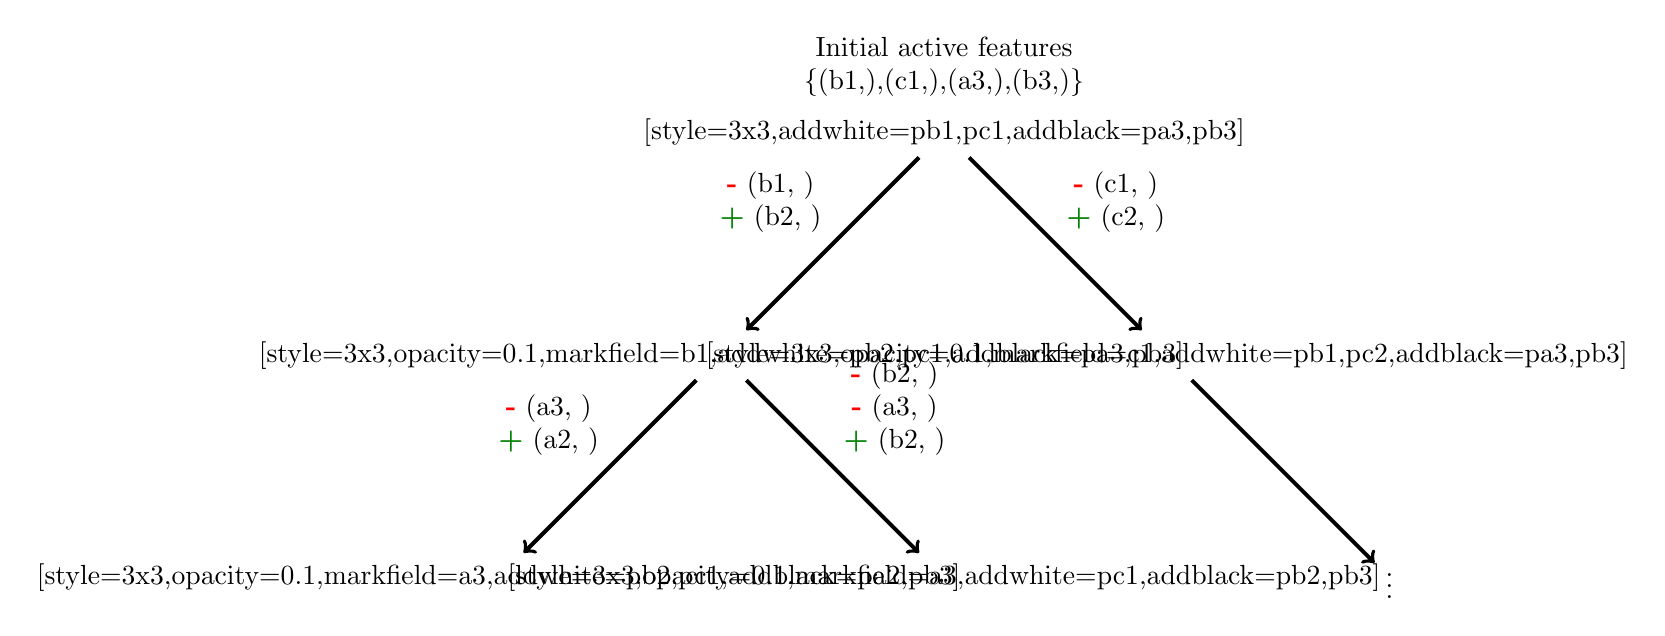
\begin{tikzpicture}[
    node distance=4cm,
    line width=0.5mm,
    auto
]

    \node[label={[align=center]Initial active features \\ \{(b1,\white),(c1,\white),(a3,\black),(b3,\black)\}}] (A) {\chessboard[style=3x3,addwhite={pb1,pc1},addblack={pa3,pb3}]};

    % childs of A
    \node (B) [below left of=A] {\chessboard[style=3x3,opacity=0.1,markfield={b1},addwhite={pb2,pc1},addblack={pa3,pb3}]};
    \node (C) [below right of=A] {\chessboard[style=3x3,opacity=0.1,markfield={c1},addwhite={pb1,pc2},addblack={pa3,pb3}]};

    % childs of B
    \node (D) [below left of=B] {\chessboard[style=3x3,opacity=0.1,markfield={a3},addwhite={pb2,pc1},addblack={pa2,pb3}]};
    \node (E) [below right of=B] {\chessboard[style=3x3,opacity=0.1,markfield={a3},addwhite={pc1},addblack={pb2,pb3}]};

    % childs of C
    \node (F) [below right of=C] {\vdots};

    % arrows of A
    \path[<-] (B) edge node[align=center] {\textbf{{\color{Red}-}} (b1, \white) \\ \textbf{{\color{Green}+}} (b2, \white)} (A);
    \path[->] (A) edge node[align=center] {\textbf{{\color{Red}-}} (c1, \white) \\ \textbf{{\color{Green}+}} (c2, \white)} (C);
    
    % arrows of B
    \path[<-] (D) edge node[align=center] {\textbf{{\color{Red}-}} (a3, \black) \\ \textbf{{\color{Green}+}} (a2, \black)} (B);
    \path[->] (B) edge node[align=center] {\textbf{{\color{Red}-}} (b2, \white) \\ \textbf{{\color{Red}-}} (a3, \black) \\ \textbf{{\color{Green}+}} (b2, \black)} (E);

    % arrows of C
    \path[<-] (F) edge node[align=center] {} (C);

\end{tikzpicture}
}
\caption{Árbol parcial de feature updates (\textcolor{Green}{agregados} y \textcolor{Red}{borrados}) para $(\featureset{Squares} \times \featureset{Colors})$ (POV blanco) en un tablero simplificado 3x3 de peones.}
\end{figure}
\end{frame}

\begin{frame}
\frametitle{\reflectbox{NNUE}: Resumen}
\begin{itemize}
\item<1-> La red son 3 capas fully connected, con parámetros $L1$ y $L2$.
\item<2-> Tenemos un acumulador de la primera capa por cada jugador.
\item<3-> Los acumuladores se actualizan eficientemente con cada movimiento, en la recursión.
\end{itemize}
\end{frame}

\begin{frame}
\frametitle{\reflectbox{NNUE}: Tradeoff}
\textbf{Tiempo de inferencia} vs. \textbf{nodos visitados}. \\
\vspace{1em}
\pause
Si la red es rápida (y por lo tanto débil), se pueden visitar más nodos y llegar más profundo. \\
\pause
Si se tienen predicciones de mayor calidad (y por lo tanto más lento), se visitan menos nodos pero con evaluaciones más precisas. \\
\pause
\vspace{1em}
\textbf{No es directo determinar qué resulta más fuerte.}
\end{frame}
